\documentclass{beamer}
% \documentclass[handout]{beamer}


%% Some packages
\usepackage{epsfig}
\usepackage{algorithmic}
\usepackage{array}
\usepackage{eurosym}
\usepackage{listings}
\lstset{basicstyle=\small\tt}
\usepackage[orientation=landscape,size=custom,width=16.8,height=10.5,scale=0.5]{beamerposter} 
%\usepackage[T1]{fontenc}


%% Some macros
\newcommand\dx{\,\mbox{d}x}


%% Table column types
\newcommand\PBS[1]{\let\temp=\\%
    #1%
    \let\\=\temp}
\newcolumntype{x}[1]
    {>{\PBS\raggedright\hspace{0pt}}p{#1}}

%% ETH font
\renewcommand{\familydefault}{let}
\renewcommand{\sfdefault}{let}
%\setbeamerfont{normal text}{family=\sffamily}


%% Colors
\xdefinecolor{grey}{rgb}{0.95,0.95,0.9375}
\xdefinecolor{myblue}{rgb}{0.664,0.762,0.867}
\xdefinecolor{myred}{rgb}{1.0,0.0,0.328}

\setbeamercolor{background canvas}{fg=black,bg=grey}
\setbeamercolor{normal text}{fg=black,bg=grey}
\setbeamercolor{itemize item}{fg=myblue}
\setbeamercolor{itemize subitem}{fg=myblue}
\setbeamercolor{itemize subsubitem}{fg=myblue}
\setbeamercolor{alert}{fg=myred}

\setbeamercolor{section in head/foot}{fg=white,bg=black}
\setbeamerfont{section in head/foot}{size=\LARGE}

\setbeamercolor{subsection in head/foot}{fg=white,bg=black}
\setbeamerfont{subsection in head/foot}{size=\normalsize}

\setbeamercolor{title in head/foot}{fg=white,bg=black}
\setbeamerfont{title in head/foot}{size=\tiny}

\setbeamercolor{date in head/foot}{fg=white,bg=black}
\setbeamerfont{date in head/foot}{size=\tiny}

\setbeamerfont{itemize subitem}{size=\normalsize}

\setbeamerfont{footnote}{size=\tiny}


%% Margins
\setbeamersize{text margin left=3ex}
\setbeamersize{text margin right=5ex}
\setbeamersize{sidebar width left=0ex}
\setbeamersize{sidebar width right=0ex}


%% Define the bullet
\setbeamertemplate{itemize item}[square]


%% Define the Headline
% \setbeamertemplate{headline}{
% \begin{beamercolorbox}[wd=0.8\paperwidth,ht=8ex,dp=2ex,leftskip=3ex]{section in head/foot}
%     \usebeamerfont{section in head/foot}\insertsection
% \end{beamercolorbox}
% \begin{beamercolorbox}[wd=0.8\paperwidth,ht=4ex,dp=3.5ex,leftskip=3ex,rightskip=3ex]{subsection in head/foot}
%     \usebeamerfont{subsection in head/foot}\insertsubsection
% \end{beamercolorbox}
% \begin{beamercolorbox}[right,wd=0.2\paperwidth,ht=12ex,dp=2ex,rightskip=3ex]{section in head/foot}
%     \includegraphics[width=10ex]{logo.pdf}
% \end{beamercolorbox}
% }
\setbeamertemplate{headline}{
\hbox{\begin{beamercolorbox}[wd=0.75\paperwidth,ht=14ex]{}
\begin{beamercolorbox}[wd=0.75\paperwidth,ht=8ex,dp=2ex,leftskip=3ex]{section in head/foot}
    \usebeamerfont{section in head/foot}\insertsection
\end{beamercolorbox}
\begin{beamercolorbox}[wd=0.75\paperwidth,ht=4ex,dp=3.5ex,leftskip=3ex,rightskip=3ex]{subsection in head/foot}
    \usebeamerfont{subsection in head/foot}\insertsubsection
\end{beamercolorbox}\end{beamercolorbox}%
\begin{beamercolorbox}[right,wd=0.25\paperwidth,ht=14ex,dp=3.5ex,rightskip=3ex]{section in head/foot}
    \vspace{-1ex}
\includegraphics[height=12ex]{DU_W_O_med.png}
\end{beamercolorbox}}
}


%% Define the Footline
\setbeamertemplate{footline}{
\hbox{\begin{beamercolorbox}[wd=0.7\paperwidth,ht=3ex,dp=1.4ex,leftskip=3ex]{title in head/foot}
    \usebeamerfont{title in head/foot} \insertauthor: \inserttitle
\end{beamercolorbox}%
\begin{beamercolorbox}[right,wd=0.3\paperwidth,ht=3ex,dp=1.4ex,rightskip=3ex]{date in head/foot}
    \usebeamerfont{date in head/foot}\insertdate\hspace{1ex}\insertframenumber/\inserttotalframenumber
\end{beamercolorbox}}
}


%% Title
\title{SWIFT: Fast algorithms for SPH on multi-core architectures}
\subtitle{Fast neighbour-finding and task-based parallelism}
\author{Pedro Gonnet}
\date{June 5th, 2013}


%% Slides
\begin{document}

    {
    \setbeamercolor{background canvas}{fg=white,bg=black}
    % \usebackgroundtemplate{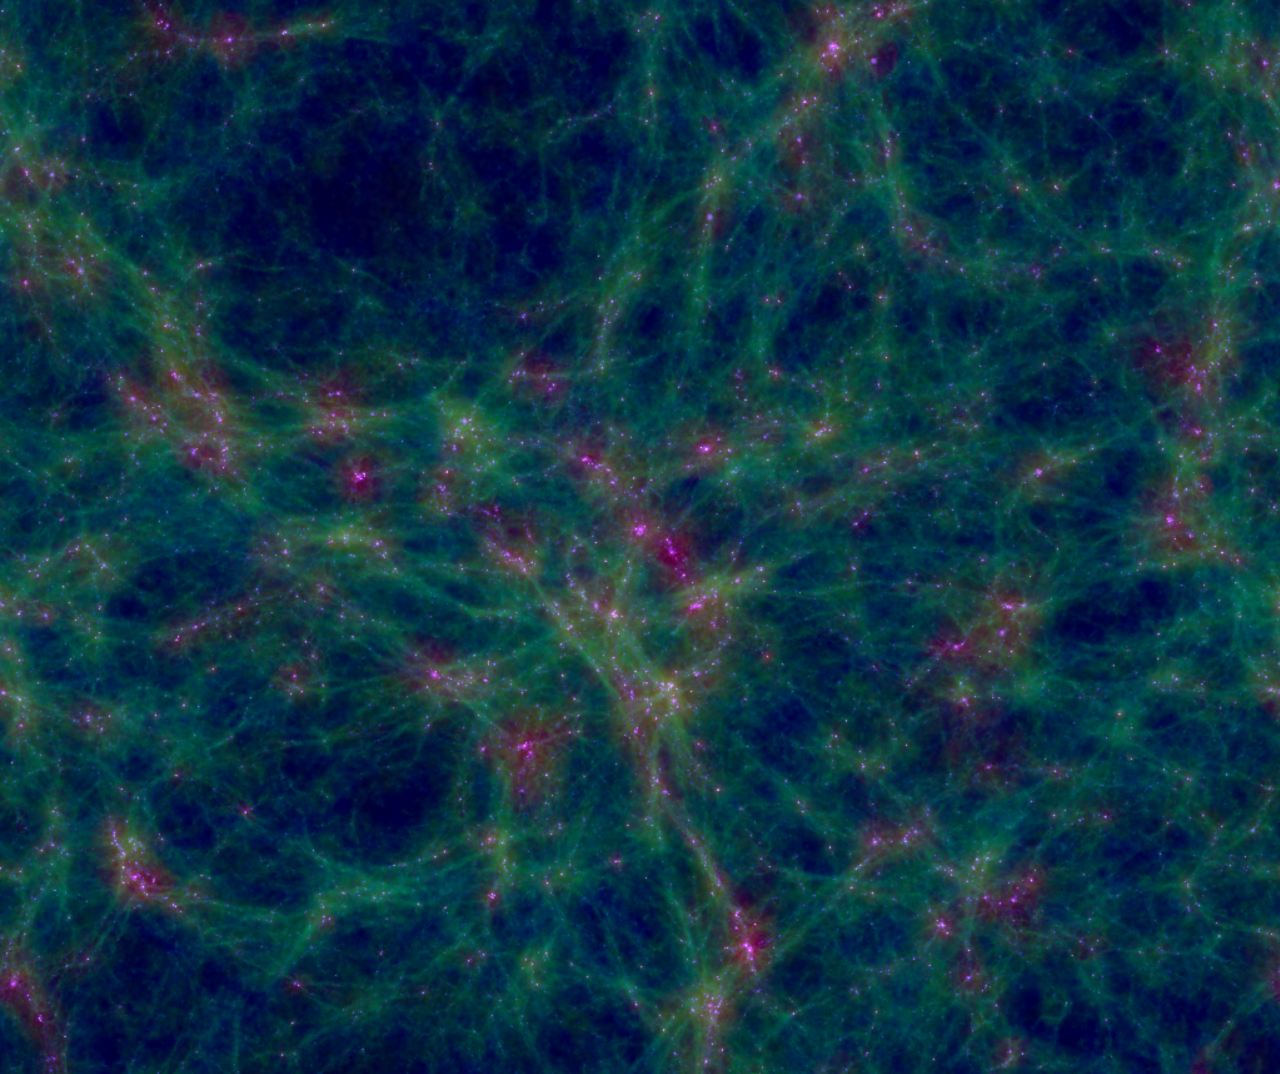
\includegraphics[width=\paperwidth]{eagle_50.png}}
        
    \section{Title}
    
    \begin{frame}[plain]
        \color{white}
        \vspace{15ex}
        {\bf\huge \inserttitle \\}
        \vspace{1.5ex}
        \Large \insertsubtitle \\
        \vspace{4ex}
        \large \insertauthor, Matthieu Schaller, Tom Theuns, Aidan Chalk \\
        \vspace{0.2ex} ECS/ICC, Durham University \\
        \vspace{0.2ex} 8th International SPHERIC Workshop, \insertdate \\
    \end{frame}
    }
    
    \setbeamercolor{background canvas}{fg=black,bg=grey}
    
    
    \section{Take-home messages}
    \subsection{What this talk is all about}
    
    \begin{frame}
        \begin{itemize}
        
            \pause
        
            \item<+-> In order to continue getting \alert<.>{\em faster}, programs
                need to become \alert<+>{\em more parallel}.
                
                % \vspace{0.5ex}
                
                \uncover<+->{$\longrightarrow$
                    If a program has reached its \alert<.>{maximum degree of parallelism},
                    it won't get any faster.} \uncover<+->{\alert<.>{Ever}.}
                
                \vspace{0.5ex}
                
            \item<+-> On shared-memory systems,
                asynchronous \alert<.>{task-based parallelism} solves most
                problems with concurrency and scaling.
                    
                % \vspace{0.5ex}
                
                \uncover<+->{$\longrightarrow$
                    But we still need to develop task-based algorithms
                    for \alert<.>{specific problems}, e.g.~SPH simulations.}
                
                \vspace{0.5ex}
                
            \item<+-> Better algorithms alone can lead to speedups
                of \alert<.>{up to a factor of ten}.
                
                % \vspace{0.5ex}
                
                \uncover<+->{$\longrightarrow$
                    Better use of both \alert<.>{existing} and \alert<+>{future}
                    infrastructure.}
                    
        \end{itemize}
    \end{frame}
        
    
    \subsection{Case in point}
    
    \begin{frame}
        \begin{itemize}
        
            \pause
        
            \item<+-> \alert<.>{Cosmological simulation} (galaxy formation) with
                \alert<+>{1.8\,M particles}
                in a cubic box of 6.25\,Mpc on a 4~$\times$ Intel Xeon X7550 with
                \alert<+>{32 cores}, 2\,GHz.
                
            \item<+-> \alert<.>{{\sc gadget}-3}, MPI-based,
               used for multi-billion particle simulations. 
                
            \item<+-> \alert<.>{\sc swift}, our own code for the same problem.
               % developed with the Institute of Computational Cosmology at
               % Durham University.
               %
               \uncover<+->{\alert<.>{13$\times$ faster} on 32 cores.}
                
        \end{itemize}
        
        \vspace{1ex}
        
        \uncover<5->{\only<-5>{\centerline{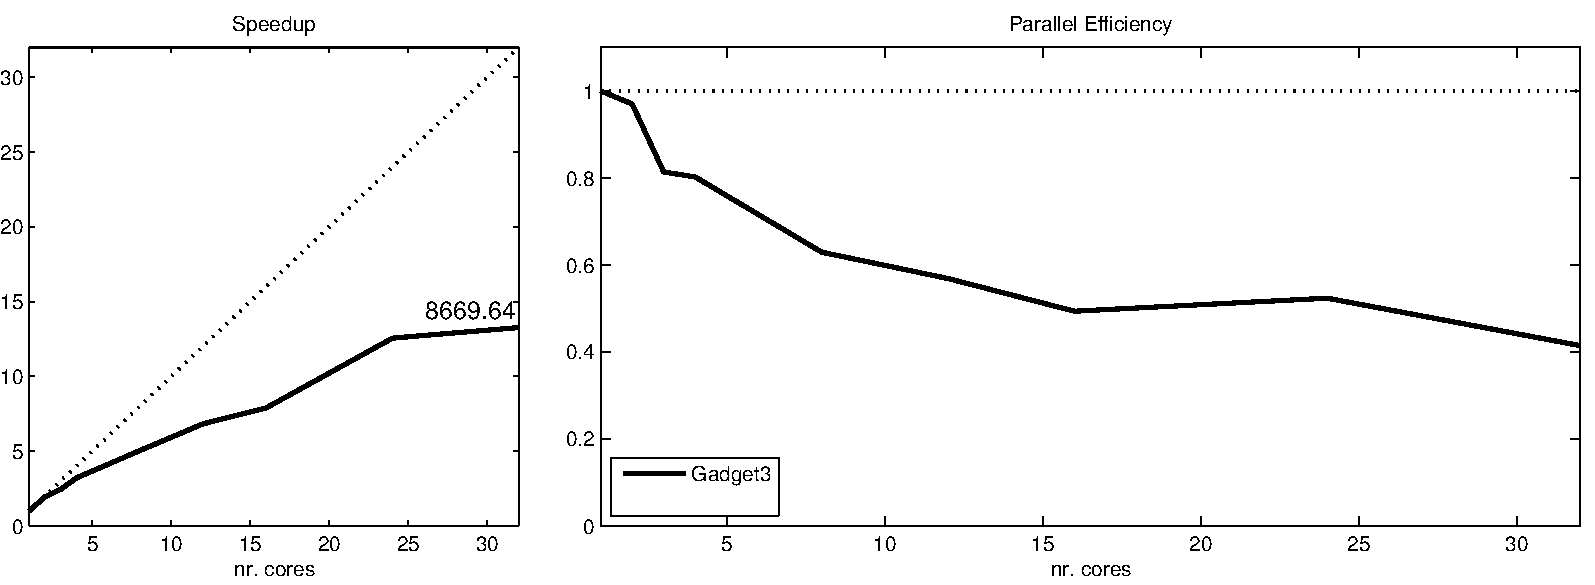
\epsfig{file=scaling_gadget.pdf, width=0.9\textwidth}}}}%
        \only<6>{\centerline{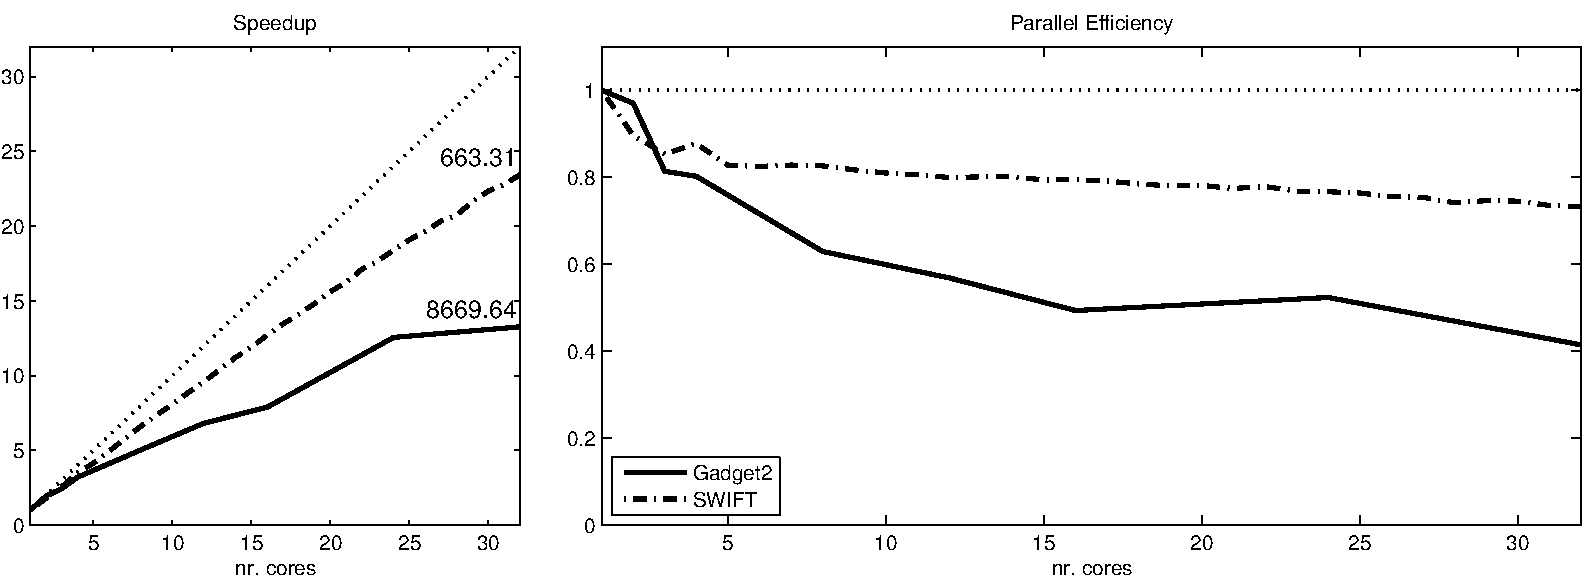
\epsfig{file=scaling.pdf, width=0.9\textwidth}}}%
        \only<7->{\centerline{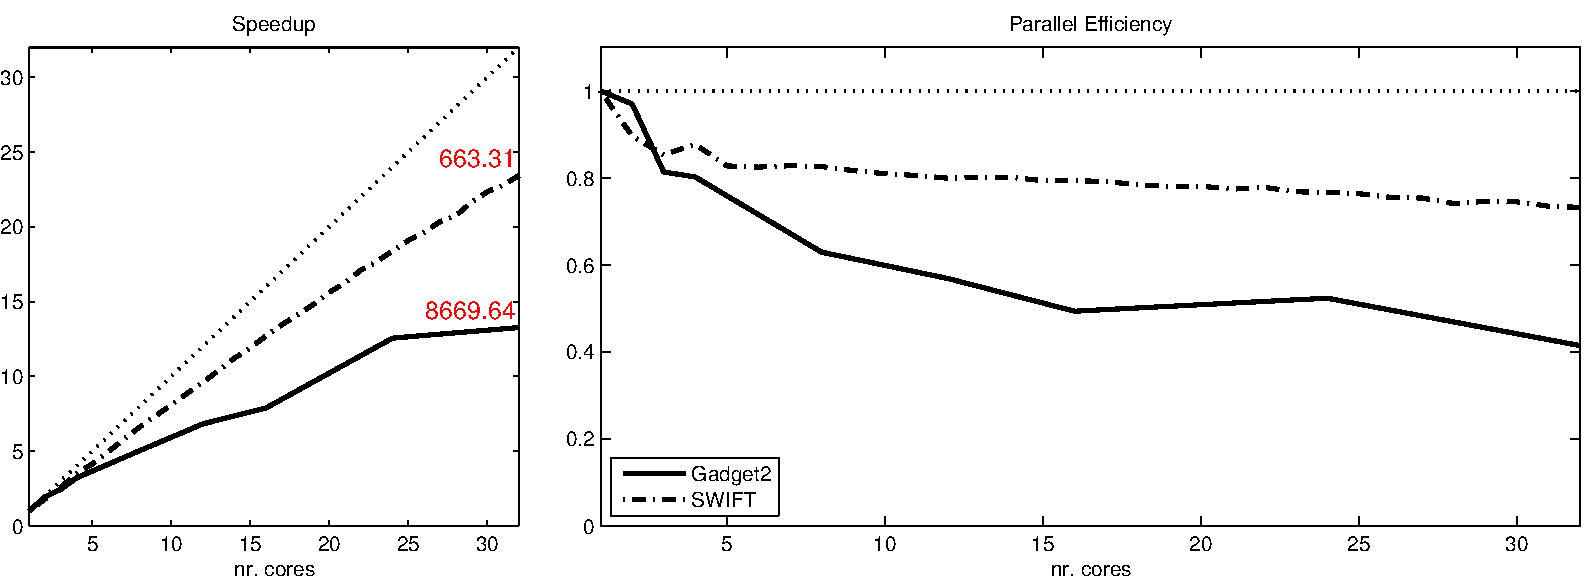
\epsfig{file=scaling_red.pdf, width=0.9\textwidth}}}%
        
    \end{frame}
    
    
    \section{Task-based parallelism}
    \subsection{Main idea}
    
    \begin{frame}
        \begin{itemize}
        
        \pause

        \item<+-> \alert<.>{Shared-memory parallel programming paradigm}
            in which the computation is formulated in an
            \alert<+>{implicitly parallelizable} way that
            automatically avoids most of the problems associated
            with \alert<+>{concurrency and load-balancing}.
            
        \end{itemize}
        
        \vspace{-1.5ex}
                
        \begin{columns}
        
            \column{0.55\textwidth}
            \begin{itemize}
            
                \item<+-> We first reduce the problem to a set of inter-dependent
                    \alert<.>{tasks}.

                \item<+-> For each task, we need to know:
                    
                    \begin{itemize}
                        \item<+-> Which tasks it \alert<.>{depends} on,
                        \item<+-> Which tasks it \alert<.>{conflicts} with.
                    \end{itemize}
                    
                \item<+-> Each thread then \alert<.>{picks up a task} which
                    has no unresolved dependencies or conflicts and computes it.
                    
            \end{itemize}
            
            \column{0.45\textwidth}
                \only<5>{\centerline{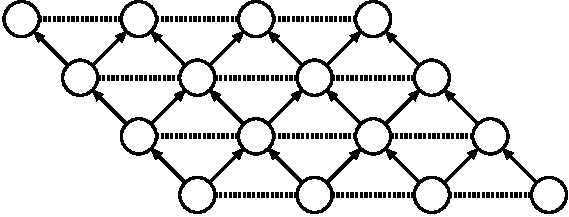
\epsfig{file=img008.pdf,width=0.9\textwidth}}}%
                \only<6>{\centerline{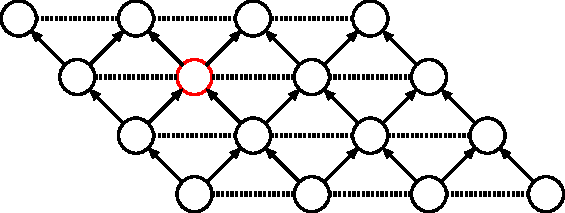
\epsfig{file=img008h.pdf,width=0.9\textwidth}}}%
                \only<7>{\centerline{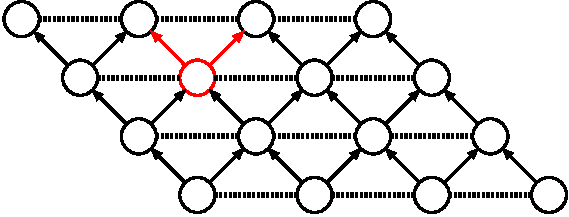
\epsfig{file=img008b.pdf,width=0.9\textwidth}}}%
                \only<8>{\centerline{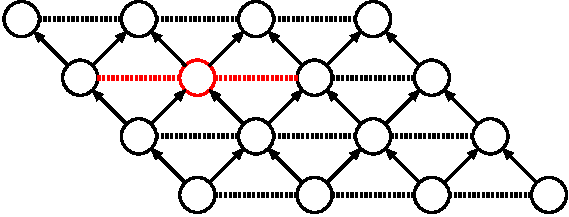
\epsfig{file=img008c.pdf,width=0.9\textwidth}}}%
                \only<9>{\centerline{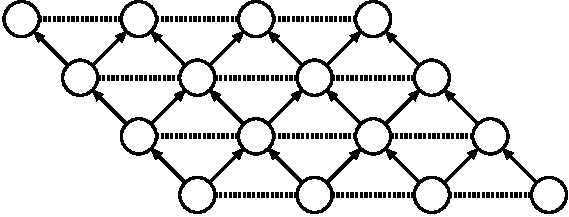
\epsfig{file=img008.pdf,width=0.9\textwidth}}}%
                \only<10>{\centerline{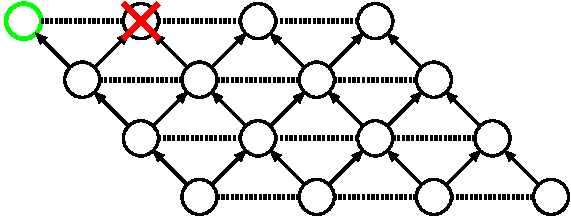
\epsfig{file=img008d.pdf,width=0.9\textwidth}}}%
                \only<11>{\centerline{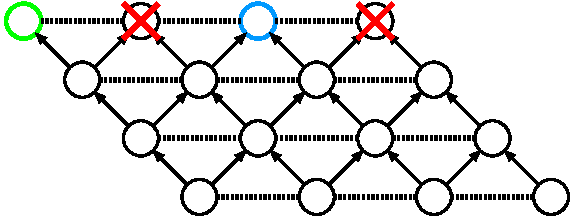
\epsfig{file=img008e.pdf,width=0.9\textwidth}}}%
                \only<12>{\centerline{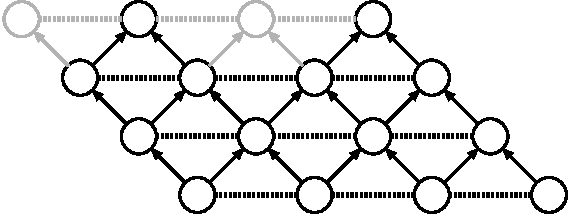
\epsfig{file=img008e2.pdf,width=0.9\textwidth}}}%
                \only<13>{\centerline{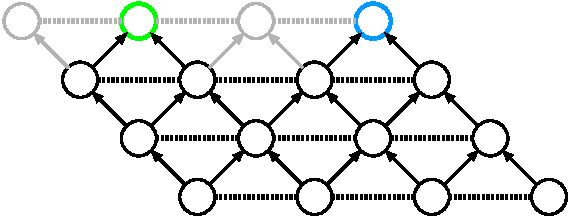
\epsfig{file=img008f.pdf,width=0.9\textwidth}}}%
                \only<14>{\centerline{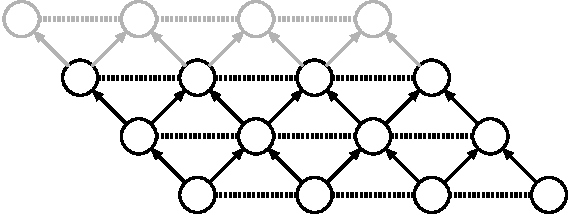
\epsfig{file=img008f2.pdf,width=0.9\textwidth}}}%
            
        \end{columns}
    \end{frame}
    
    
    \subsection{Main advantages}
    
    \begin{frame}
        \begin{itemize}
        
            \pause
            
            \item<+-> The order in which the tasks are processed is
                \alert<.>{dynamic} and
                adapts automatically to load imbalances.
                
            \item<+-> If the dependencies and conflicts are specified correctly,
                we \alert<.>{do not have to worry about concurrency} at the level
                of the individual tasks.
                
                \uncover<+->{$\longrightarrow$ No need for expensive
                    \alert<.>{explicit}
                    locking, synchronization, or atomic operations.}
                    
            \item<+-> Each task has exclusive access to the data it
                is working on, thus \alert<.>{improving cache efficiency}.
            
            \item<+-> The same approach can be applied to more
                \alert<.>{unconventional many-core systems} such as GPUs.
            
            \item<+-> However, this usually means that
                we have to \alert<.>{re-think our entire computation},
                e.g.~redesign it from scratch to make it task-based.
                
        \end{itemize}
    \end{frame}
    
    
    \section{Task-based algorithms for SPH}
    \subsection{Neighbour-finding with trees}
    
    \begin{frame}
    
        \pause
    
        \begin{columns}
        
            \column{0.65\textwidth}
            \begin{itemize}

                \item<+-> In multi-resolution SPH,
                    \alert<.>{\alert<+>{Spatial trees}} are the most commonly used
                    approach to neighbour-finding, as the particle distribution
                    can be irregular.
                    
                \item<+-> Neighbour-finding up and down the tree is
                    \alert<.>{\alert<+>{simple}}, but has some problems:
                    
                    \begin{itemize}
                        \item<+-> Worst-case cost in 
                            \alert<.>{$\mathcal O(N^{2/3})$} per particle.
                        \item<+-> \alert<.>{Low cache efficiency} due to scattered
                            memory access.
                        \item<+-> Symmetries cannot be exploited, i.e.~each
                            particle pair is \alert<.>{found twice}.
                    \end{itemize}
                    
                \item<+-> Parallelization is \alert<.>{trivial}, but only because
                    symmetries are not exploited.

            \end{itemize}
            
            \column{0.35\textwidth}
                \only<2>{\centerline{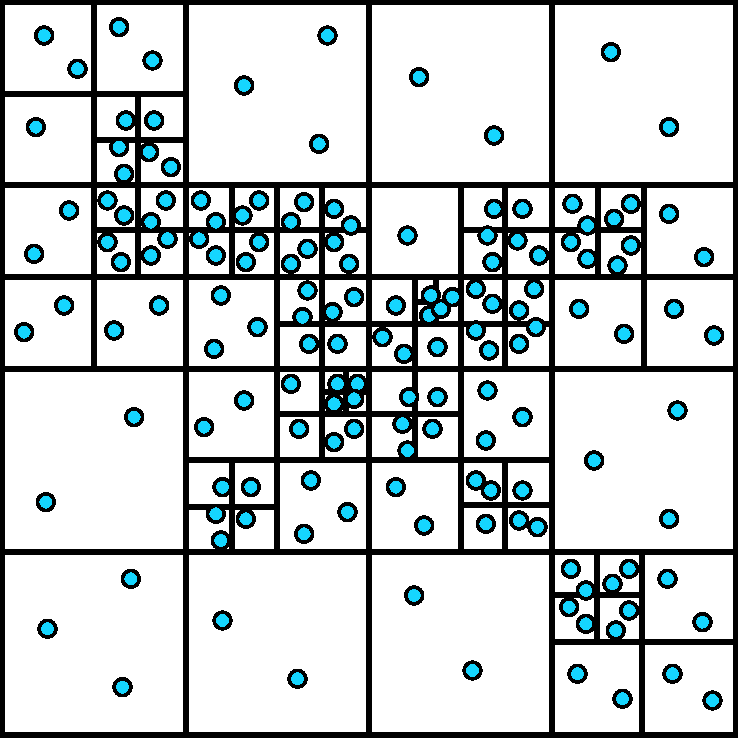
\epsfig{file=Octree.pdf,width=0.8\textwidth}}}%
                \only<3>{\centerline{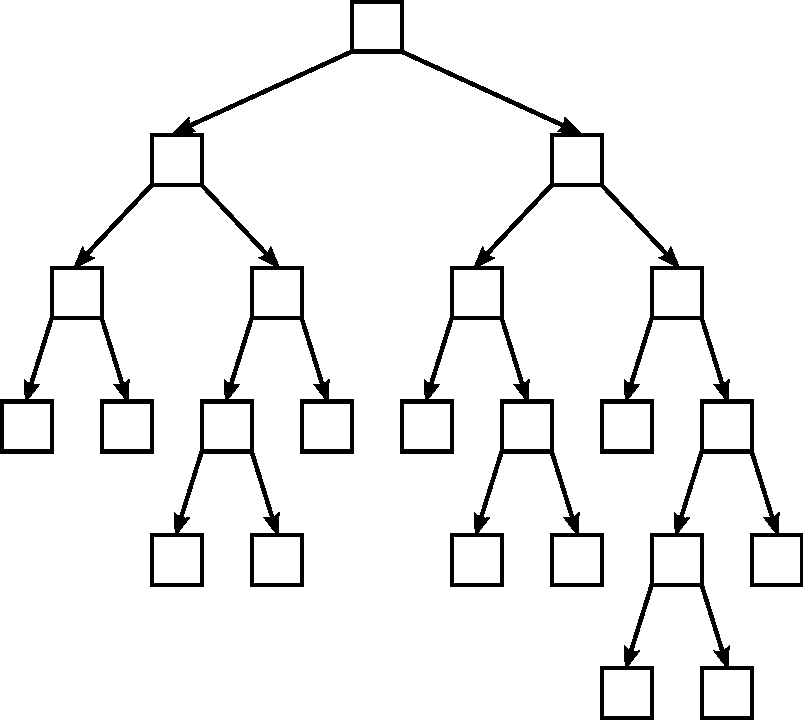
\epsfig{file=SearchTree_001.pdf,width=0.8\textwidth}}}%
                \only<4>{\centerline{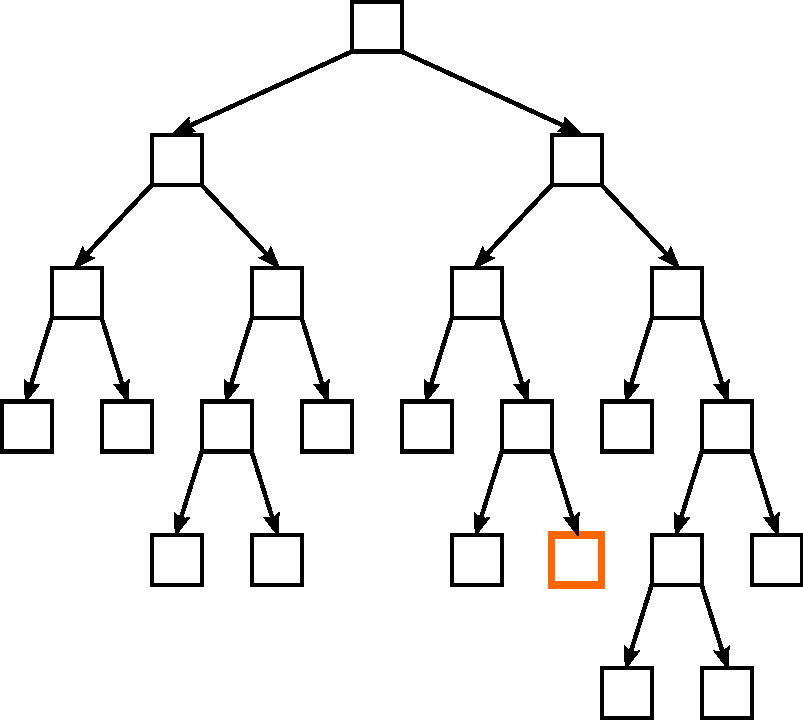
\epsfig{file=SearchTree_002.pdf,width=0.8\textwidth}}}%
                \only<5->{\centerline{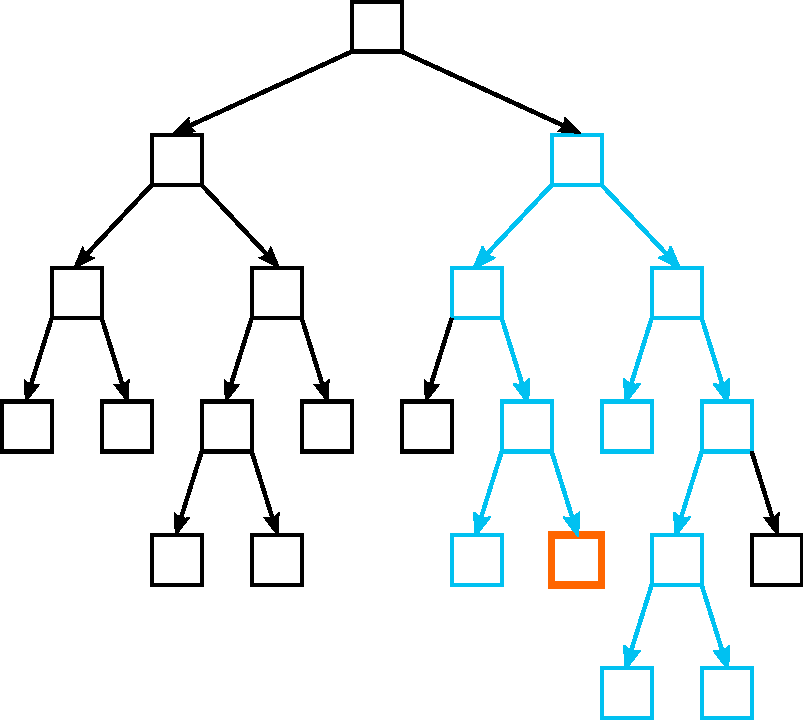
\epsfig{file=SearchTree_003.pdf,width=0.8\textwidth}}}%
            
        \end{columns}
    \end{frame}
    
    
    \subsection{Hierarchical cell pairs}
    
    \begin{frame}
    
        \pause

        \begin{columns}
        
            \column{0.65\textwidth}
            \begin{itemize}

                \item<+-> We start by splitting the simulation domain into
                    rectangular \alert<.>{cells} of edge length at least
                    $h_\mathsf{max}$.
                    
                \item<+-> All interacting particle pairs are then in either
                    in the \alert<.>{same cell}, or in a
                    \alert<+>{pair of neighbouring cells}.
                    
                \item<+-> Finding \alert<.>{all neighbours} within each cell
                    or between each
                    pair of cells can be used as a \alert<+>{task}.
                    %
                    \uncover<+->{$\longrightarrow$ Instead of traversing
                        the tree for each particle, we \alert<.>{traverse a list of
                        cells and cell pairs} and compute all interactions.}
                    
            \end{itemize}
            
            \column{0.35\textwidth}
                \only<2>{\centerline{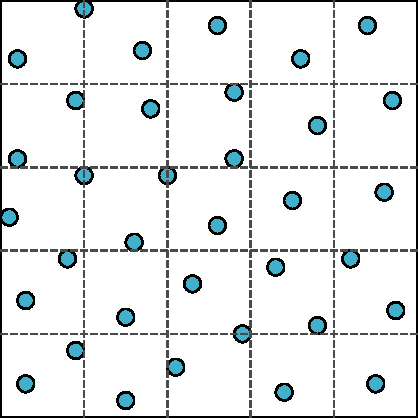
\epsfig{file=InitialDecomp_001.pdf,width=0.8\textwidth}}}%
                \only<3-4>{\centerline{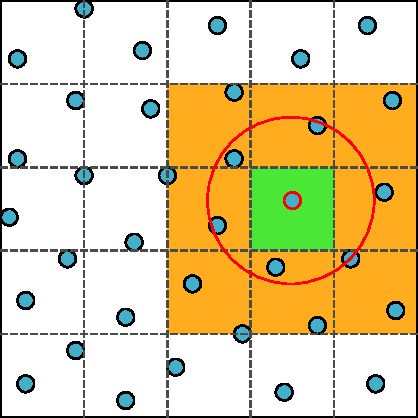
\epsfig{file=InitialDecomp_002.pdf,width=0.8\textwidth}}}%
                \only<5-7>{\centerline{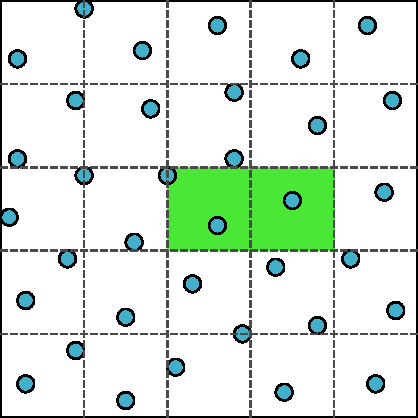
\epsfig{file=InitialDecomp_004.pdf,width=0.8\textwidth}}}%
         
        \end{columns}
    \end{frame}
    
    
    \begin{frame}
    
        \begin{columns}
        
            \column{0.65\textwidth}
            \begin{itemize}
            
                \item<+-> In a mutli-resolution setting, the initial
                    cell-based decomposition can be \alert<.>{extremely
                    inefficient}.
                    
                \item<+-> If the particles in a cell 
                    are sufficiently small, the self-interaction task
                    can be \alert<.>{split}.
                    
                \item<+-> Likewise, if the particles in a cell-pair 
                    are sufficiently small, the task
                    can be \alert<.>{split} as well.
                    
                \item<+-> Finally, the particles in each cell pair are
                    \alert<.>{first sorted} along the cell pair axis to speed-up
                    neighbour-finding.

            \end{itemize}
            
            \column{0.35\textwidth}
                \only<2>{\centerline{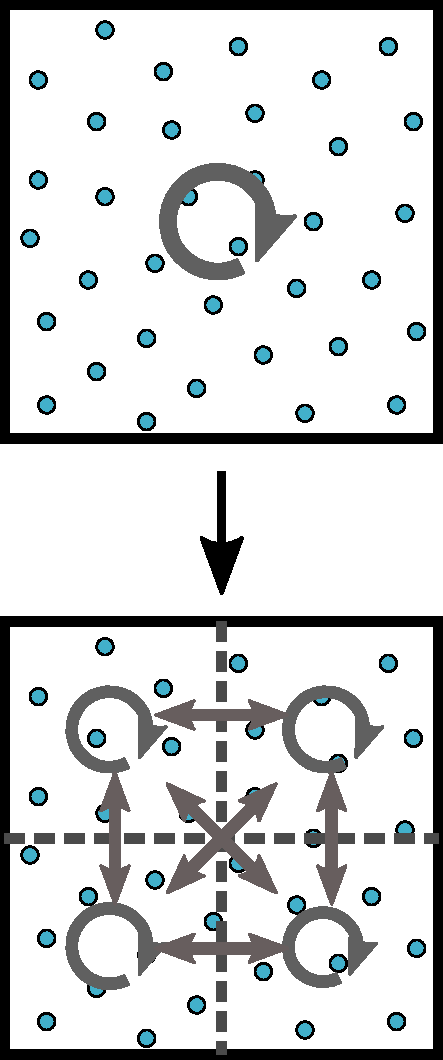
\epsfig{file=SplitCell.pdf,width=0.4\textwidth}}}%
                \only<3>{\centerline{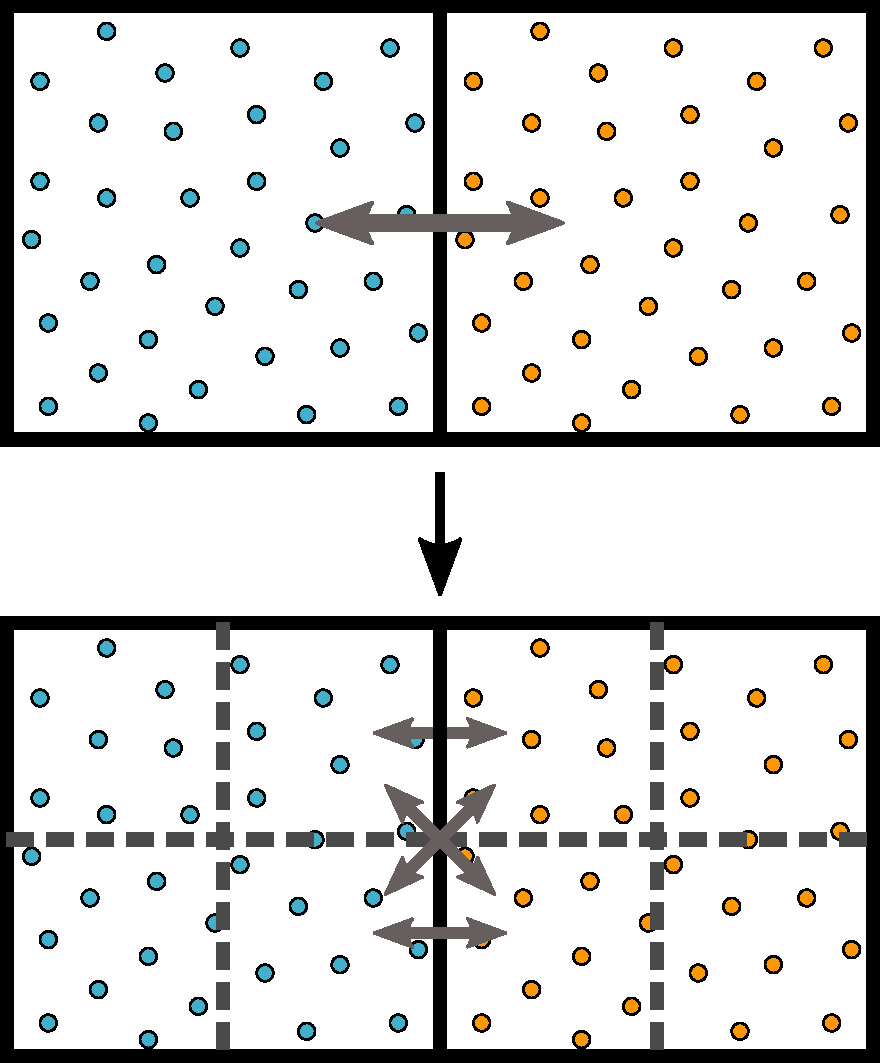
\epsfig{file=SplitPair.pdf,width=0.8\textwidth}}}%
                \only<4>{\centerline{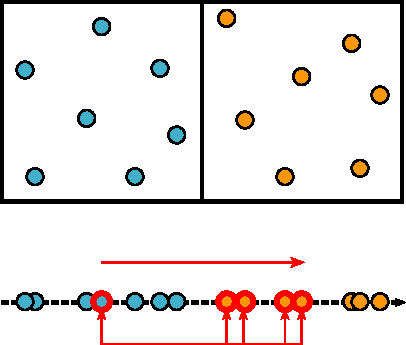
\epsfig{file=SortedInteractions.pdf,width=0.8\textwidth}}}%
         
        \end{columns}
    \end{frame}
    
    
    \subsection{Task hierarchy}
    
    \begin{frame}
    
        \pause

        \begin{columns}
        
            \column{0.65\textwidth}
            \begin{itemize}

                \item<+-> \alert<.>{Three main task types}: \alert<+>{Sorting},
                    \alert<+>{self-interactions},
                    and \alert<+>{pair-interactions}.
                    
                \item<+-> \alert<.>{``Ghost'' tasks} are added to group dependencies
                    between the density and force tasks of each cell.
                    
                \item<+-> Each \alert<.>{sorting task} depends on the sorting tasks
                    of its sub-cells (merge-sort).
                    
                \item<+-> Each \alert<.>{pair-interaction} task depends on the sort tasks
                    of the cells involved.
                    
                \item<+-> Tasks on \alert<.>{overlapping cells conflict}, i.e.~they can
                    not execute concurrently.

            \end{itemize}
            
            \column{0.35\textwidth}
                \only<2>{\centerline{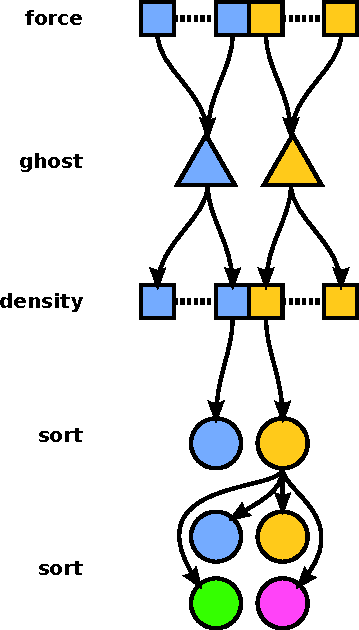
\epsfig{file=Hierarchy2.pdf,height=0.8\textheight}}}%
                \only<3>{\centerline{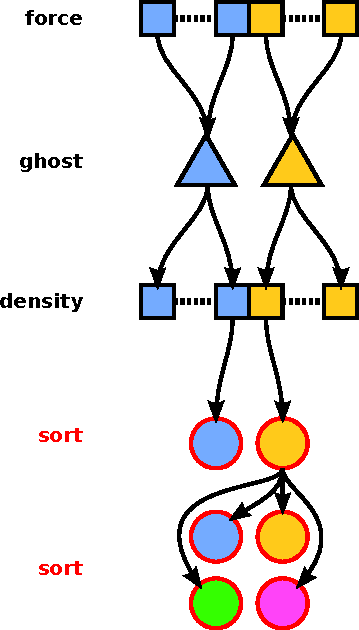
\epsfig{file=Hierarchy2_005.pdf,height=0.8\textheight}}}%
                \only<4>{\centerline{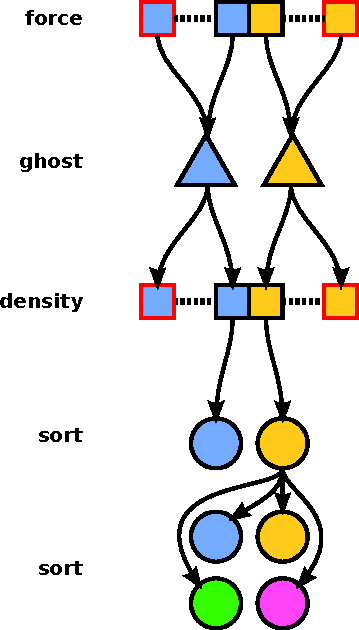
\epsfig{file=Hierarchy2_007.pdf,height=0.8\textheight}}}%
                \only<5>{\centerline{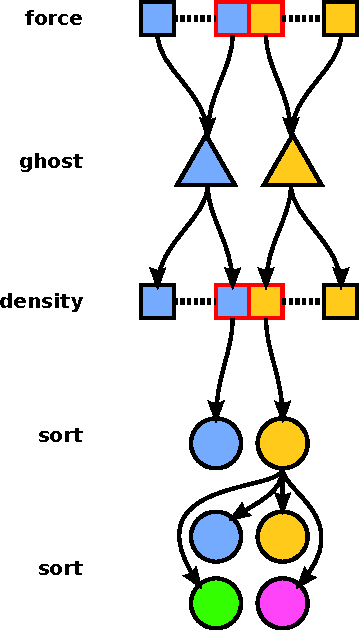
\epsfig{file=Hierarchy2_006.pdf,height=0.8\textheight}}}%
                \only<6>{\centerline{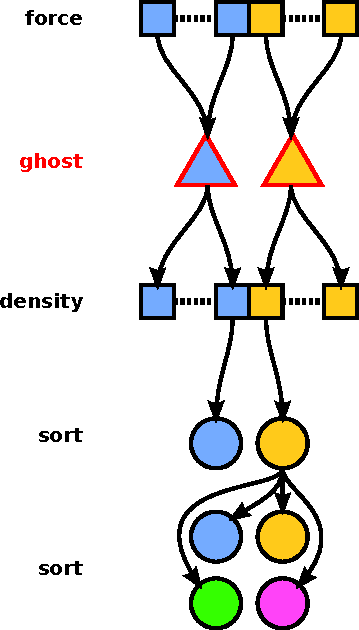
\epsfig{file=Hierarchy2_008.pdf,height=0.8\textheight}}}%
                \only<7>{\centerline{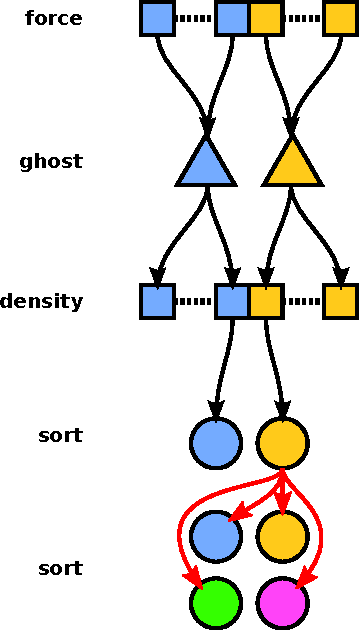
\epsfig{file=Hierarchy2_001.pdf,height=0.8\textheight}}}%
                \only<8>{\centerline{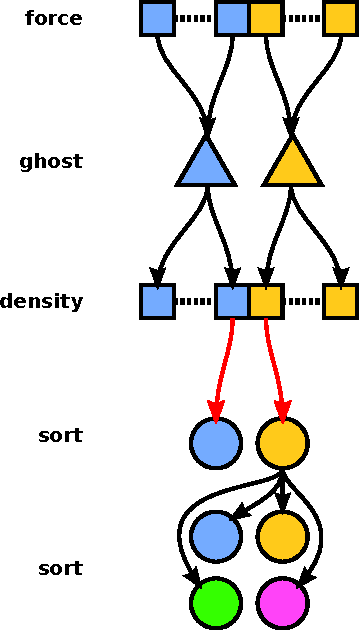
\epsfig{file=Hierarchy2_002.pdf,height=0.8\textheight}}}%
                \only<9>{\centerline{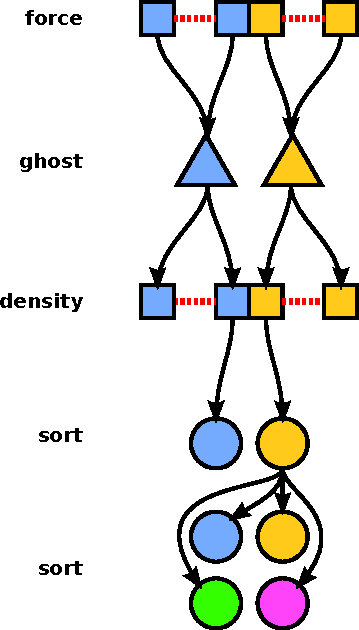
\epsfig{file=Hierarchy2_004.pdf,height=0.8\textheight}}}%
         
        \end{columns}
    \end{frame}
    
    
    \subsection{Dynamic task allocation}
    
    \begin{frame}
    
        \centerline{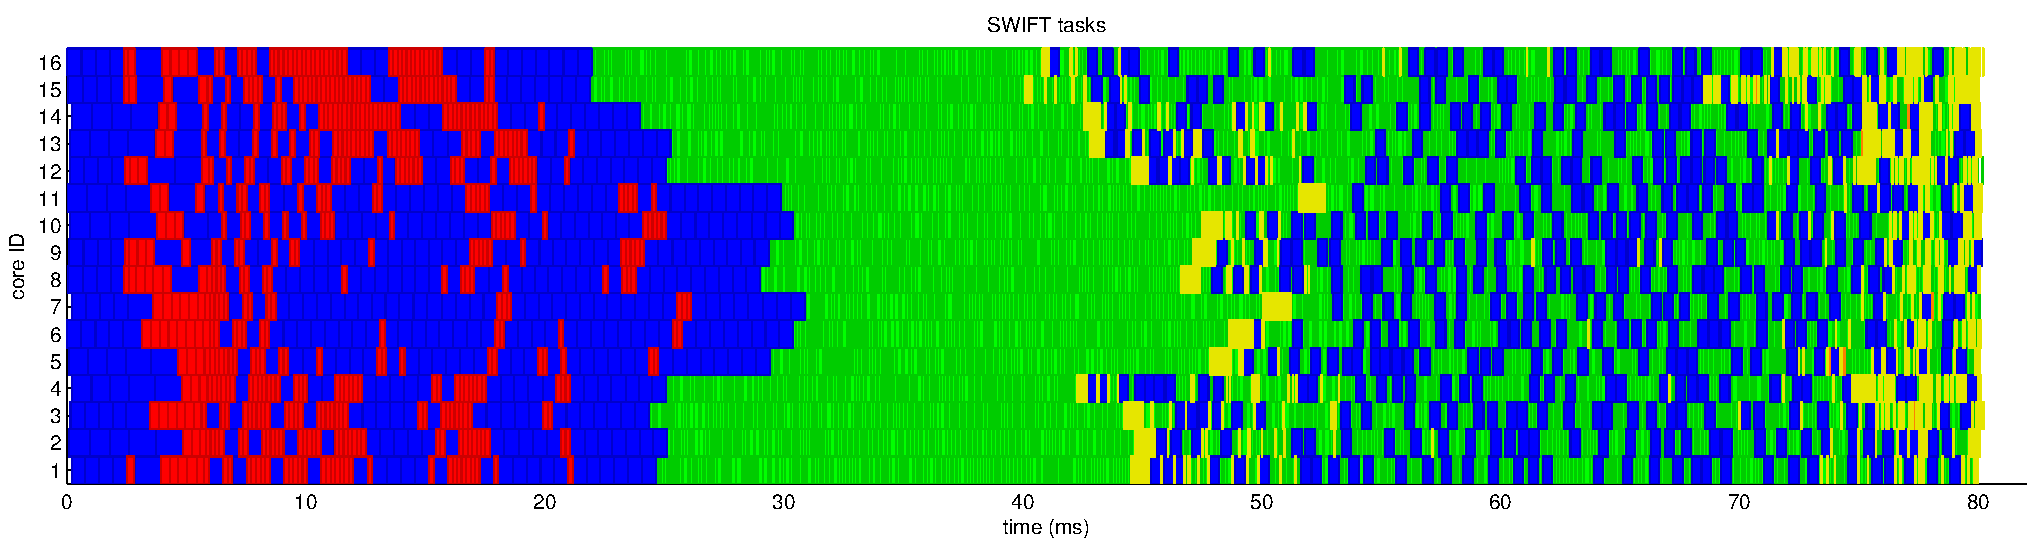
\epsfig{file=tasks_dynamic.pdf,width=\textwidth}}
        
        \pause
        
        \begin{itemize}
        
            \item<+-> Each core has it's own task queue and uses
                \alert<.>{work-stealing} when empty.
                
            \item<+-> Each core has a \alert<.>{preference} for tasks involving
                cells which were used previously to improve cache re-use.

        \end{itemize}
    \end{frame}
    
    
    \subsection{Parallel efficiency and scaling}
    
    \begin{frame}
    
        \pause
        
        \centerline{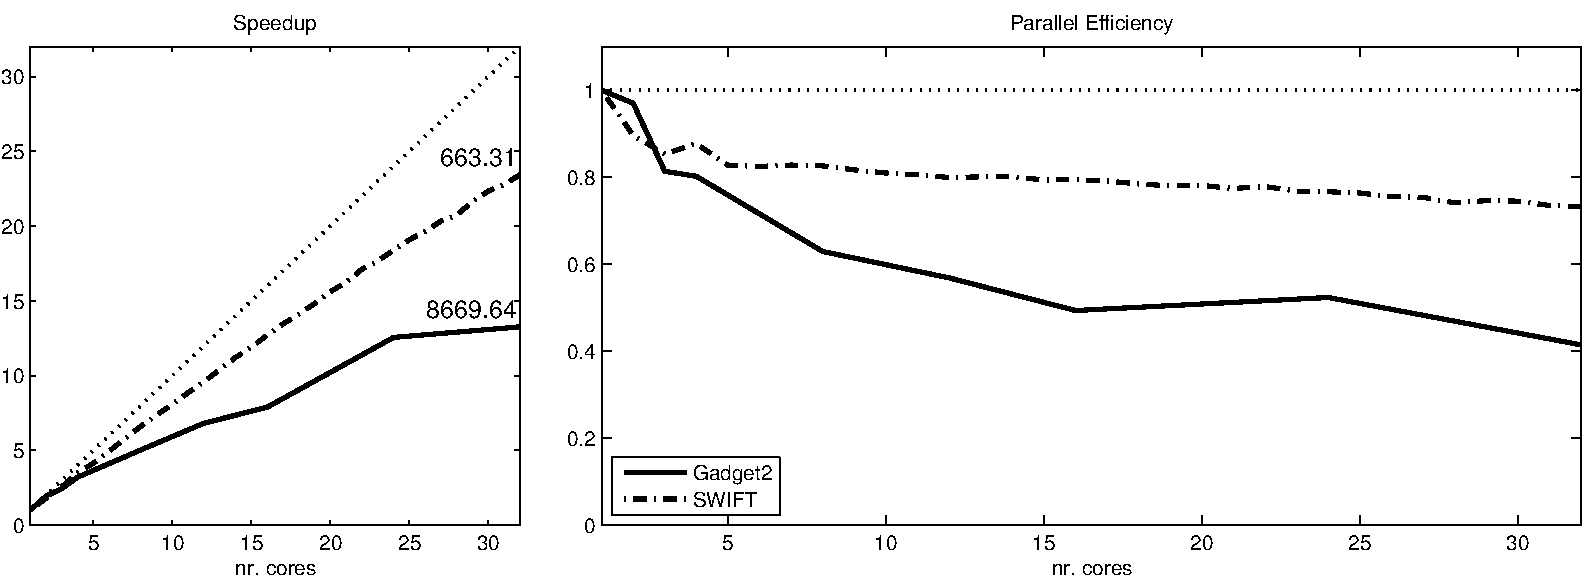
\epsfig{file=scaling.pdf,width=0.8\textwidth}}
        
        \pause
        
        \begin{itemize}
        
            \item<+-> Parallel efficiency of \alert<.>{$75\%$} on 32 cores of
                an $4\times$ Intel Xeon X7550 shared-memory machine.
                
            \item<+-> \alert<.>{No NUMA-related effects}: Each
                task operates exclusively on a small contiguous region
                of memory which usually
                fits in the \alert<+>{lower level caches}.

        \end{itemize}
    \end{frame}
    
    
    \subsection{Further work}
    
    \begin{frame}
        \begin{itemize}
        
            \pause
            
            \item<+-> {\sc swift} is currently an Open-Source \alert<.>{research
                code}, but we aim to be able to do \alert<+>{production runs}
                in Computational Cosmology.
                
            \item<+-> \alert<.>{Modular structure}, easy to add
                new physics, kernel functions, etc\dots
        
            \item<+-> \alert<.>{Hybrid} shared/distributed-memory parallelism:
            
                \begin{itemize}
                    \item<+-> \alert<.>{Distributed-memory parallelism} between the
                        nodes of a cluster,.
                    \item<+-> \alert<.>{Task-based shared-memory parallelism} between
                        the cores of a single node.
                    \item<+-> \alert<.>{SIMD/SIMT parallelism} within each task
                        on a single core.
                \end{itemize}
                
            \item<+-> In a task-based hybrid setup, sending and receiving
                data asynchronously can be implemented as tasks to
                \alert<.>{hide communication latencies}.
                
            \item<+-> \alert<.>{Mixed-precision floating point arithmetic}
                in order to better exploit SIMD vectorization, yet
                \alert<+>{without losing precision}.
                
            \item<+-> Tasks can also be \alert<.>{shared between the
                CPU and a GPU}.
                
        \end{itemize}
    \end{frame}
    
    
    \section{Conclusions}
    \subsection{Take-home messages}
    
    \begin{frame}
        \begin{itemize}
        
            \item<+-> In order to continue getting {\em faster}, programs
                need to become {\em more parallel}.
                
                % \vspace{0.5ex}
                
                $\longrightarrow$
                    If a program has reached its maximum degree of parallelism,
                    it won't get any faster. Ever.
                
                \vspace{0.5ex}
                
            \item On shared-memory systems,
                asynchronous task-based parallelism solves most
                problems with concurrency and scaling.
                    
                % \vspace{0.5ex}
                
                $\longrightarrow$
                    But we still need to develop task-based algorithms
                    for specific problems, e.g.~SPH simulations.
                
                \vspace{0.5ex}
                
            \item Better algorithms alone can lead to speedups
                of up to a factor of ten.
                
                % \vspace{0.5ex}
                
                $\longrightarrow$
                    Better use of both existing and future
                    infrastructure.
                    
            \item<+-> If you have an \alert<.>{interesting problem}, or
                just need a \alert<+>{fast code}, let us know!
                    
        \end{itemize}
    \end{frame}
        
    
    \subsection{Thanks}
    
    \begin{frame}
        \centerline{Thank you for your attention!}
    \end{frame}


\end{document}
